\documentclass[a4paper, 10pt, notumble]{leaflet}
\usepackage{grawlix}
\usepackage{enumitem}
\usepackage{calc}
\usepackage{array}

\usepackage[type={CC}, version={4.0}, modifier={by}]{doclicense} % Add text and icons for creative commons license

\usepackage[hidelinks]{hyperref} % Add hyperlinks to the pdf file. This should usually be the last package loaded before \begin{document}


\newcommand{\smallat}{{\setmainfont{Comic Neue-Bold} \Large @}}
\newcommand{\smallpound}{{\setmainfont{Comic Neue-Bold} \large \#}}
\newcommand{\smalldollar}{{\setmainfont{Comic Neue-Bold} \large \$}}
\newcommand{\smallpercent}{{\setmainfont{Comic Neue-Bold} \large \%}}
\newcommand{\smallampersand}{{\setmainfont{Comic Neue-Bold} \large \$}}
\newcommand{\smallasterisk}{{\setmainfont{Quicksand-Bold} \Huge \raisebox{-0.25ex}{\textasteriskcentered{}}}}

\newlength{\glen}
\newlength{\rlen}
\newlength{\alen}
\newlength{\wlen}
\newlength{\llen}
\newlength{\ilen}

\begin{document}

{
\begin{center}
\setmainfont{Quicksand-Medium}
\footnotesize
Version 0.1
\end{center}

\begin{center}
\setmainfont[Scale=2.175]{Cooper Black}
\Huge Grawlix
\end{center}

%{
%\begin{center}
%\setmainfont[Scale=1.66]{Cooper Black}
%\Huge
%\setlength{\glen}{\widthof{G}/2 + \widthof{r}/2 + 8pt}
%\setlength{\rlen}{\glen + \widthof{r}/2 + \widthof{a}/2 + 8pt}
%\setlength{\alen}{\rlen + \widthof{a}/2 + \widthof{w}/2 + 8pt}
%\setlength{\wlen}{\alen + \widthof{w}/2 + \widthof{l}/2 + 8pt}
%\setlength{\llen}{\wlen + \widthof{l}/2 + \widthof{i}/2 + 8pt}
%\setlength{\ilen}{\llen + \widthof{i}/2 + \widthof{x}/2 + 8pt}
%
%\contourlength{0.25mm}
%\begin{tikzpicture}
%\node[tile, inner sep = 3pt] () at (0,0) {\rule[-0.25ex]{0pt}{1.875ex}\contour{black}{\textcolor{red}{G}}};
%\node[tile, inner sep = 3pt] () at (\glen,0) {\rule[-0.25ex]{0pt}{1.875ex}\contour{black}{\textcolor{orange}{r}}};
%\node[tile, inner sep = 3pt] () at (\rlen,0) {\rule[-0.25ex]{0pt}{1.875ex}\contour{black}{\textcolor{yellow}{a}}};
%\node[tile, inner sep = 3pt] () at (\alen,0) {\rule[-0.25ex]{0pt}{1.875ex}\contour{black}{\textcolor{green}{w}}};
%\node[tile, inner sep = 3pt] () at (\wlen,0) {\rule[-0.25ex]{0pt}{1.875ex}\contour{black}{\textcolor{blue}{l}}};
%\node[tile, inner sep = 3pt] () at (\llen,0) {\rule[-0.25ex]{0pt}{1.875ex}\contour{black}{\textcolor{violet}{i}}};
%\node[tile, inner sep = 3pt] () at (\ilen,0) {\rule[-0.25ex]{0pt}{1.875ex}\contour{black}{\textcolor{red}{x}}};
%
%\end{tikzpicture}
%
%\end{center}
%}
\begin{center}
\setmainfont{Quicksand-Medium}
\huge The Typesetters' Game%A Tale of Two Typesetters
\end{center}

\vfill%\vspace{1.0cm}

\begin{center}
\begin{tikzpicture}[transform shape, scale=2.5]

\foreach \i/\j/\k in {0.0/blue/at, 0.5/violet/ampersand, 1.0/yellow/dollar, 1.5/green/asterisk, 2.0/red/octothorpe, 2.5/orange/percent} {
	\node[tile] () at (\i,0.0) {};
	\pic () at (\i,0.0) {\k={\j}};
}

\foreach \i/\j/\k in {0.0/orange/asterisk, 0.5/red/dollar, 1.0/violet/at, 1.5/blue/ampersand, 2.0/yellow/percent, 2.5/green/octothorpe} {
	\node[tile] () at (\i,-0.5) {};
	\pic () at (\i,-0.5) {\k={\j}};
}

\foreach \i/\j/\k in {0.0/violet/percent, 0.5/blue/octothorpe, 1.0/red/asterisk, 1.5/orange/dollar, 2.0/green/at, 2.5/yellow/ampersand} {
	\node[tile] () at (\i,-1.0) {};
	\pic () at (\i,-1.0) {\k={\j}};
}

\foreach \i/\j/\k in {0.0/green/dollar, 0.5/yellow/asterisk, 1.0/blue/percent, 1.5/violet/octothorpe, 2.0/orange/ampersand, 2.5/red/at} {
	\node[tile] () at (\i,-1.5) {};
	\pic () at (\i,-1.5) {\k={\j}};
}

\foreach \i/\j/\k in {0.0/red/ampersand, 0.5/green/percent, 1.0/orange/octothorpe, 1.5/yellow/at, 2.0/blue/asterisk} {
	\node[tile] () at (\i,-2.0) {};
	\pic () at (\i,-2.0) {\k={\j}};
}

\foreach \i/\j/\k in {0.0/yellow/octothorpe, 0.5/orange/at, 1.0/green/ampersand, 1.5/red/percent} {
	\node[tile] () at (\i,-2.5) {};
	\pic () at (\i,-2.5) {\k={\j}};
}

\node[tile, rotate=15] () at (1.25,-3.575) {};
\pic[rotate=15] () at (1.25, -3.575) {dollar={violet}};

\node[tile, rotate=-30] () at (2.25,-3.575) {};
\pic[rotate=-30] () at (2.25, -3.575) {dollar={blue}};

\node[tile, rotate=30] () at (0.25,-3.575) {};
\pic[rotate=30] () at (0.25, -3.575) {asterisk={violet}};
\end{tikzpicture}

\end{center}

\vfill

\begin{center}
\setmainfont{Quicksand-Medium}
\huge Michael Purcell\\
Dannielle Harden
\end{center}
}
\newpage
\setmainfont{Quicksand}[
	UprightFont = *-Medium,
	BoldFont = *-Bold]
\raggedright

\section{Overview}
Grawlix is a game for two players that can be played in 15 \textendash 30 minutes. It is suitable for all ages, but is intended for players who are eight years old or older.

Grawlix is a version of the typesetters' game (see the last page of this leaflet). The gameplay is the same but the components are a bit different. In this version, plastic tiles are used in place of metal type. Also, different colors are used to distinguish tiles instead of different typefaces.

\section{Components}
To play Grawlix, the players will need a flat \textbf{play area} and thirty-six \textbf{tiles}. Each tile is labelled with one of six possible \textbf{glyphs} and one of six possible \textbf{colors}.  There is one tile for each possible combination of glyph and color.

The six glyphs are: \smallat, \smallpound, \smalldollar, \smallpercent, \smallampersand, \smallasterisk. The six colors are: red, orange, yellow, green, blue, violet.

\begin{figure}[h]
\centering
\begin{tikzpicture}[transform shape, scale=2.5]
\foreach \i / \j in {0 / red, -0.5 / orange, -1.0 / yellow, -1.5 / green, -2.0 / blue, -2.5 / violet} {
\node[tile] () at (0,\i) {};
\pic () at (0,\i) {at={\j}};
\node[tile] () at (0.5,\i) {};
\pic () at (0.5,\i) {octothorpe={\j}};
\node[tile] () at (1,\i) {};
\pic () at (1,\i) {dollar={\j}};
\node[tile] () at (1.5,\i) {};
\pic () at (1.5,\i) {percent={\j}};
\node[tile] () at (2,\i) {};
\pic () at (2,\i) {ampersand={\j}};
\node[tile] () at (2.5,\i) {};
\pic () at (2.5,\i) {asterisk={\j}};
}

\end{tikzpicture}

\end{figure}

\newpage

\section{The Grid}
During the game, the players will place tiles in the play area. These tiles will be organized into a \textbf{grid} made up of \textbf{rows} and \textbf{columns}. A row is a group of tiles that are on the same horizontal line.  A column is a group of tiles that are on the same vertical line. The grid should have no more than six rows and six columns.

A \textbf{line} is a generic term that can refer to either a single row or a single column of the grid. Each line can contain no more than one tile with each glyph and one tile with each color.

\subsection{Notes}
At the beginning of the game, the grid is empty.

Rows and columns do not need to be contiguous.
If two tiles are on the same line then they must have different glyphs and colors.

\section{Set Up}
The tiles should be placed face up to one side of the play area. These tiles comprise the \textbf{supply}. The supply should be arranged in a square. Each column should have all tiles of a given glyph and each row should have all tiles of a given color.

The players should decide which one of them will be the \textbf{first player}.

Starting with the first player, the players then take turns \textbf{drafting} tiles. To draft a tile, a player should choose one tile from the supply and add that tile to their \textbf{hand}.

The set up phase is complete when both players have drafted four tiles.

\subsection{Notes}
All tiles should be visible to both players at all times.  This includes the supply, the grid, and both players' hands.

\newpage

\section{Gameplay}
The players should take turns playing tiles from their hands until one of them is unable to do so.

After playing each tile the current player should draft a tile to replace the tile that they played. If there are no tiles in the supply, then they should skip this step.

If a player is unable to play a tile on their turn then that player loses the game.

\subsection{Playing Tiles}
On their first turn, the first player should play a tile from their hand by placing it face up anywhere in the play area. This tile is the first tile in the grid.

On later turns, the current player should play a tile from their hand by placing it face up next to a tile in the grid. After it is played, this tile becomes part of the grid.

When a new tile is played it must be placed in the play area such that:
\begin{enumerate}
  \item At least one edge of the new tile is aligned with an edge of another tile in the grid.
  \item The glyph of the new tile is different from the glyph of every other tile in the:
  \begin{enumerate}
  	\item row in which it is placed.
    	\item column in which it is placed.
  \end{enumerate}
  \item The color of the new tile is different from the color of every other tile in the:
  \begin{enumerate}
  	\item row in which it is placed.
    \item column in which it is placed.
  \end{enumerate}
  \item The grid has no more than six rows and six columns.
\end{enumerate}

\newpage

\section{Example}
%In the following example,
%it is early in the game. Three tiles are in the grid: the red \smallampersand, the blue \smallpound, and the yellow \smallasterisk.  The next player can place their tile in one of seven possible locations. These locations are indicated by the dotted squares in the diagram below.
%
%\begin{figure}[h]
%\centering
%%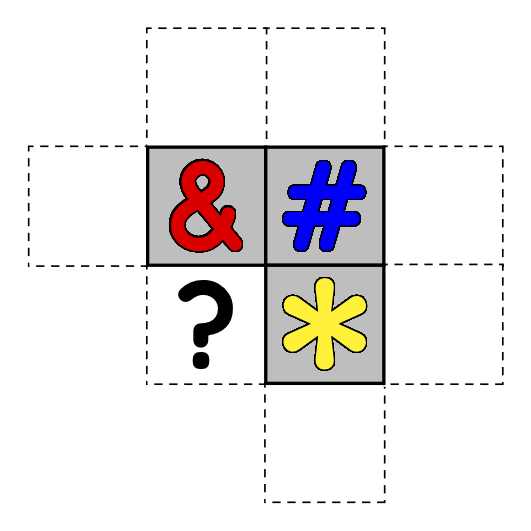
\includegraphics[scale=0.275]{Images/small_example.png}
%\begin{tikzpicture}[transform shape, scale=2.5]
%
%\node[vacant] () at (-0.5,0) {};
%\node[dotter] () at (-0.5,0) {};
%
%\node[vacant] () at (0.5,0.5) {};
%\node[dotter, rotate=180] () at (0.5,0.5) {};
%
%\node[vacant] () at (0,0.5) {};
%\node[dotter] () at (0,0.5) {};
%
%\node[vacant] () at (0,-0.5) {};
%\node[dotter] () at (0,-0.5) {\Large{?}};
%
%\node[vacant] () at (0.5,-1) {};
%\node[dotter] () at (0.5,-1) {};
%
%\node[vacant] () at (1,0) {};
%\node[dotter, rotate=180] () at (1,0) {};
%
%\node[vacant] () at (1,-0.5) {};
%\node[dotter, rotate=180] () at (1,-0.5) {};
%
%\node[tile] () at (0,0) {};
%\pic () at (0,0) {ampersand={red}};
%\node[tile] () at (0.5,0) {};
%\pic () at (0.5,0) {octothorpe={blue}};
%\node[tile] () at (0.5,-0.5) {};
%\pic () at (0.5,-0.5) {asterisk={yellow}};
%
%\end{tikzpicture}
%
%\end{figure}
%
%Consider the location labelled with the question mark. The only tile in this column is the red \smallampersand\ and the only tile in this row is the yellow \smallasterisk. So, the allowed glyphs and colors for a tile placed in this location are:
%\begin{description}[labelindent=0.25cm, itemsep=0pt]
%  \item[Glyphs:] \smallat, \smallpound, \smalldollar, \smallpercent.
%  \item[Colors:] orange, green, blue, or violet.
%\end{description}
%During the game, more tiles will be added to the grid. This will further restrict which tiles can be placed in each location.
%
Seventeen tiles are in the grid. The next player can place their tile in one of sixteen possible locations. These locations are indicated by the dotted squares in the diagram below.

The grid has six columns, so a tile cannot be placed in a new column. The grid only has five rows, so a tile can be placed in a new row.

\begin{figure}[h]
\centering
%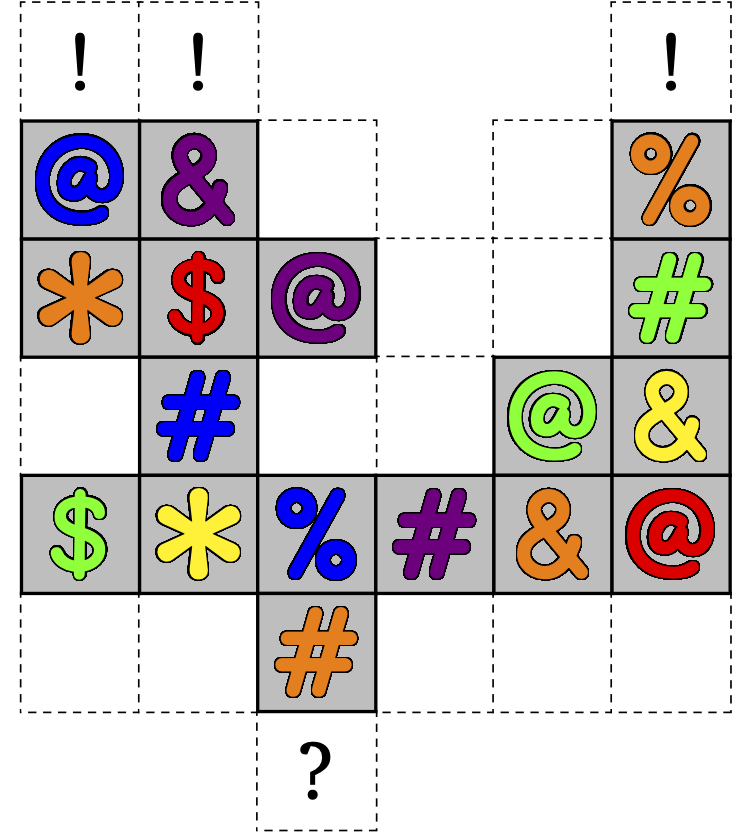
\includegraphics[scale=0.275]{Images/big_example.png}
\begin{tikzpicture}[transform shape, scale=2.5]

\node[vacant] at (0,0.5) {};
\node[dotter] at (0,0.5) {\Large{?}};
\node[vacant] at (0.5,0.5) {};
\node[dotter, rotate=180] at (0.5,0.5) {};
\node[vacant] at (2.5,0.5) {};
\node[dotter, rotate=180] at (2.5,0.5) {};

\node[vacant] at (1,0) {};
\node[dotter, rotate=180] at (1,0) {};
\node[vacant] at (2,0) {};
\node[dotter] at (2,0) {};
\node[vacant] at (1.5,-0.5) {};
\node[dotter] at (1.5,-0.5) {};
\node[vacant] at (2,-0.5) {};
\node[dotter] at (2,-0.5) {};
\node[vacant] at (1.5,-1) {};
\node[dotter] at (1.5,-1) {};

\node[vacant] at (0,-1) {};
\node[dotter] at (0,-1) {};
\node[vacant] at (1,-1) {};
\node[dotter] at (1,-1) {};

\node[vacant] at (0,-2) {};
\node[dotter] at (0,-2) {};
\node[vacant] at (0.5,-2) {};
\node[dotter] at (0.5,-2) {};
\node[vacant] at (1.5,-2) {};
\node[dotter] at (1.5,-2) {};
\node[vacant] at (2,-2) {};
\node[dotter] at (2,-2) {};
\node[vacant] at (2.5,-2) {};
\node[dotter] at (2.5,-2) {};

\node[vacant] at (1,-2.5) {};
\node[dotter] at (1,-2.5) {\Large{!}};


\foreach \i/\j/\k in {0.0/blue/at, 0.5/violet/ampersand, 2.5/orange/percent} {
	\node[tile] () at (\i,0.0) {};
	\pic () at (\i,0.0) {\k={\j}};
}

\foreach \i/\j/\k in {0.0/orange/asterisk, 0.5/red/dollar, 1.0/violet/at, 2.5/green/octothorpe} {
	\node[tile] () at (\i,-0.5) {};
	\pic () at (\i,-0.5) {\k={\j}};
}

\foreach \i/\j/\k in {0.5/blue/octothorpe, 2.0/green/at, 2.5/yellow/ampersand} {
	\node[tile] () at (\i,-1.0) {};
	\pic () at (\i,-1.0) {\k={\j}};
}

\foreach \i/\j/\k in {0.0/green/dollar, 0.5/yellow/asterisk, 1.0/blue/percent, 1.5/violet/octothorpe, 2.0/orange/ampersand, 2.5/red/at} {
	\node[tile] () at (\i,-1.5) {};
	\pic () at (\i,-1.5) {\k={\j}};
}

\foreach \i/\j/\k in {1.0/orange/octothorpe} {
	\node[tile] () at (\i,-2.0) {};
	\pic () at (\i,-2.0) {\k={\j}};
}

\end{tikzpicture}

\end{figure}

Consider the location labelled with the question mark. There are no tiles in this row. The tiles in this column are the blue \smallat, orange \smallasterisk, and green \smalldollar. So, the allowed glyphs are: \smallpound, \smallpercent, \smallampersand. The allowed colors are: red, yellow, violet.

If a tile is placed in the location labelled with the question mark, then the grid will have six rows. If that happens, then future tiles cannot be placed in a new row. In particular, the location labelled with the exclamation point will become unavailable.


\newpage

\section{The Typesetters' Game}
A pair of typesetters once worked for a local newspaper. Every Sunday, they produced a set of comic strips. This was challenging because it was so different from their regular work. In particular, the cartoonists sometimes used strings of punctuation to replace profanity. The typesetters often had to improvise to find enough type to print those sections. So, they set aside the type that they used for this purpose in a special case. Over time, they amassed a collection of thirty-six pieces of type. They had one for each of six punctuation marks in each of six typefaces.

One day, while preparing that week's comics, they noticed a curious phenomenon. They had arranged their collection of type in a square on their workbench. It was easy to ensure that every row and column had only one of each punctuation mark. It was easy to ensure that every row and column had only one of each typeface. Despite their best efforts, they could not find a way to do both at the same time.

They turned this puzzle into a game that they could play as they worked. Both players would grab a handful of type at the beginning of the day. Then, they would take turns playing by placing those pieces on the workbench. They had to place each piece next to a piece that had been played earlier. This created a grid of tiles that grew as they played. Each row and column of the grid could have only one of each punctuation mark and one of each typeface. The grid could have no more than six rows and six columns.

The game continued in this way until one player was unable to find a legal move. That player would be the loser of the game and would have to come in early the next morning to make coffee.

\vfill

\textbf{Contact}: \href{mailto:grawlix.board.game@gmail.com}{grawlix.board.game@gmail.com}

\begin{tabular}{@{}m{\textwidth-\widthof{\Huge{\doclicenseIcon}}}@{}m{\widthof{\Huge{\doclicenseIcon}}}@{}}
\footnotesize{This work is licensed under a Creative Commons\newline ``Attribute 4.0 International'' license.} & \Huge{\doclicenseIcon} \\
\end{tabular}

\end{document}